\documentclass[oneside,a4paper,11pt,explicit]{book}
\usepackage[utf8]{inputenc}
\usepackage{icecream}
\usepackage[english]{babel}
\addto\captionsenglish{\renewcommand{\chaptername}{}}
\usepackage[accsupp]{axessibility}  % improves PDF readability for those with disabilities.
\usepackage[colorlinks = true,urlcolor  = blue,linkcolor = blue]{hyperref}
\usepackage{setspace}
\usepackage{listings}
\usepackage[most]{tcolorbox}
\usepackage{minitoc}


\renewcommand{\mtifont}{\large\sffamily}
\renewcommand{\mtcfont}{\small\sffamily}
\renewcommand{\mtcSfont}{\small\sffamily}
\renewcommand{\mtcSSfont}{\small\sffamily}
\renewcommand{\mtcSSSfont}{\small\sffamily}
\mtcsetpagenumbers{minitoc}{off} % turn off page numbering in minitocs
\addto{\captionsenglish}{% Making babel aware of special titles
	\renewcommand{\mtctitle}{Quick Links To Sections}
}
\setlength{\fboxrule}{5pt}
\setlength{\fboxsep}{4pt}

\definecolor{IceCreamLeaf}{rgb}{0.4, 0.639215686274, 0.4}
\definecolor{IceCreamOrbit}{rgb}{0.803921568627451, 0.3607843137254902, 0.3607843137254902}

\title{I.C.E.C.R.E.A.M. Tutorials}
\subtitle{\small Observing Earth from Above (Env 329) - Fall 2023  \\
	\small Schmid College of Science and Technology, Chapman University}
\date{\today}

\setstretch{1.25}
\makeatletter
\begin{document}
	
	\dominitoc
	
	%\tableofcontents %%%%% After the tutorial is written, run LaTeX with this uncommented. Then comment and rerun. The mini table of contents that creates the "Quick Links To Sections" needs the toc output. 
	
	\setcounter{chapter}{3} %Insert (Tutorial Number-1) Here; example for tutorial 4, enter 3
	
	\chapter{Tutorial Name} %Enter Tutorial Name Here
	
	\vspace{-2em}
	
	\minitoc
	
	\hrule
	
	\vspace{1em}
	
	\begin{tcolorbox}[enhanced,frame style image=blueshade.png,
		opacityback=0.75,opacitybacktitle=0.25,
		colback=blue!5!white,colframe=blue!75!black,title={\Large \textbf{Objectives:}}]
		\large
		\begin{enumerate}
			\item The Learning Objective For The Tutorial Goes Here
		\end{enumerate}
	\end{tcolorbox}
	
	\clearpage
	
	%%%%%%%%%%%%%%%%%%%%%%%%%%%%%%%%%% Change Header to Have a Smaller Logo for Remainder of the Document
	\fancyhead{}
	\fancyhead[C]{\begin{tikzpicture}[overlay, remember picture]
			\fill[Blue2] (current page.north west) rectangle ($(current page.north east)+(0,-1in)$);
			\node[anchor=north west, text=white, font=\Large, minimum size=1in, inner xsep=5mm, align=left] at (current page.north west) {\bf{\MakeUppercase{\@title}}\\\@subtitle};
			\node[anchor=north east, minimum size=1in, inner xsep=5mm] at (current page.north east) {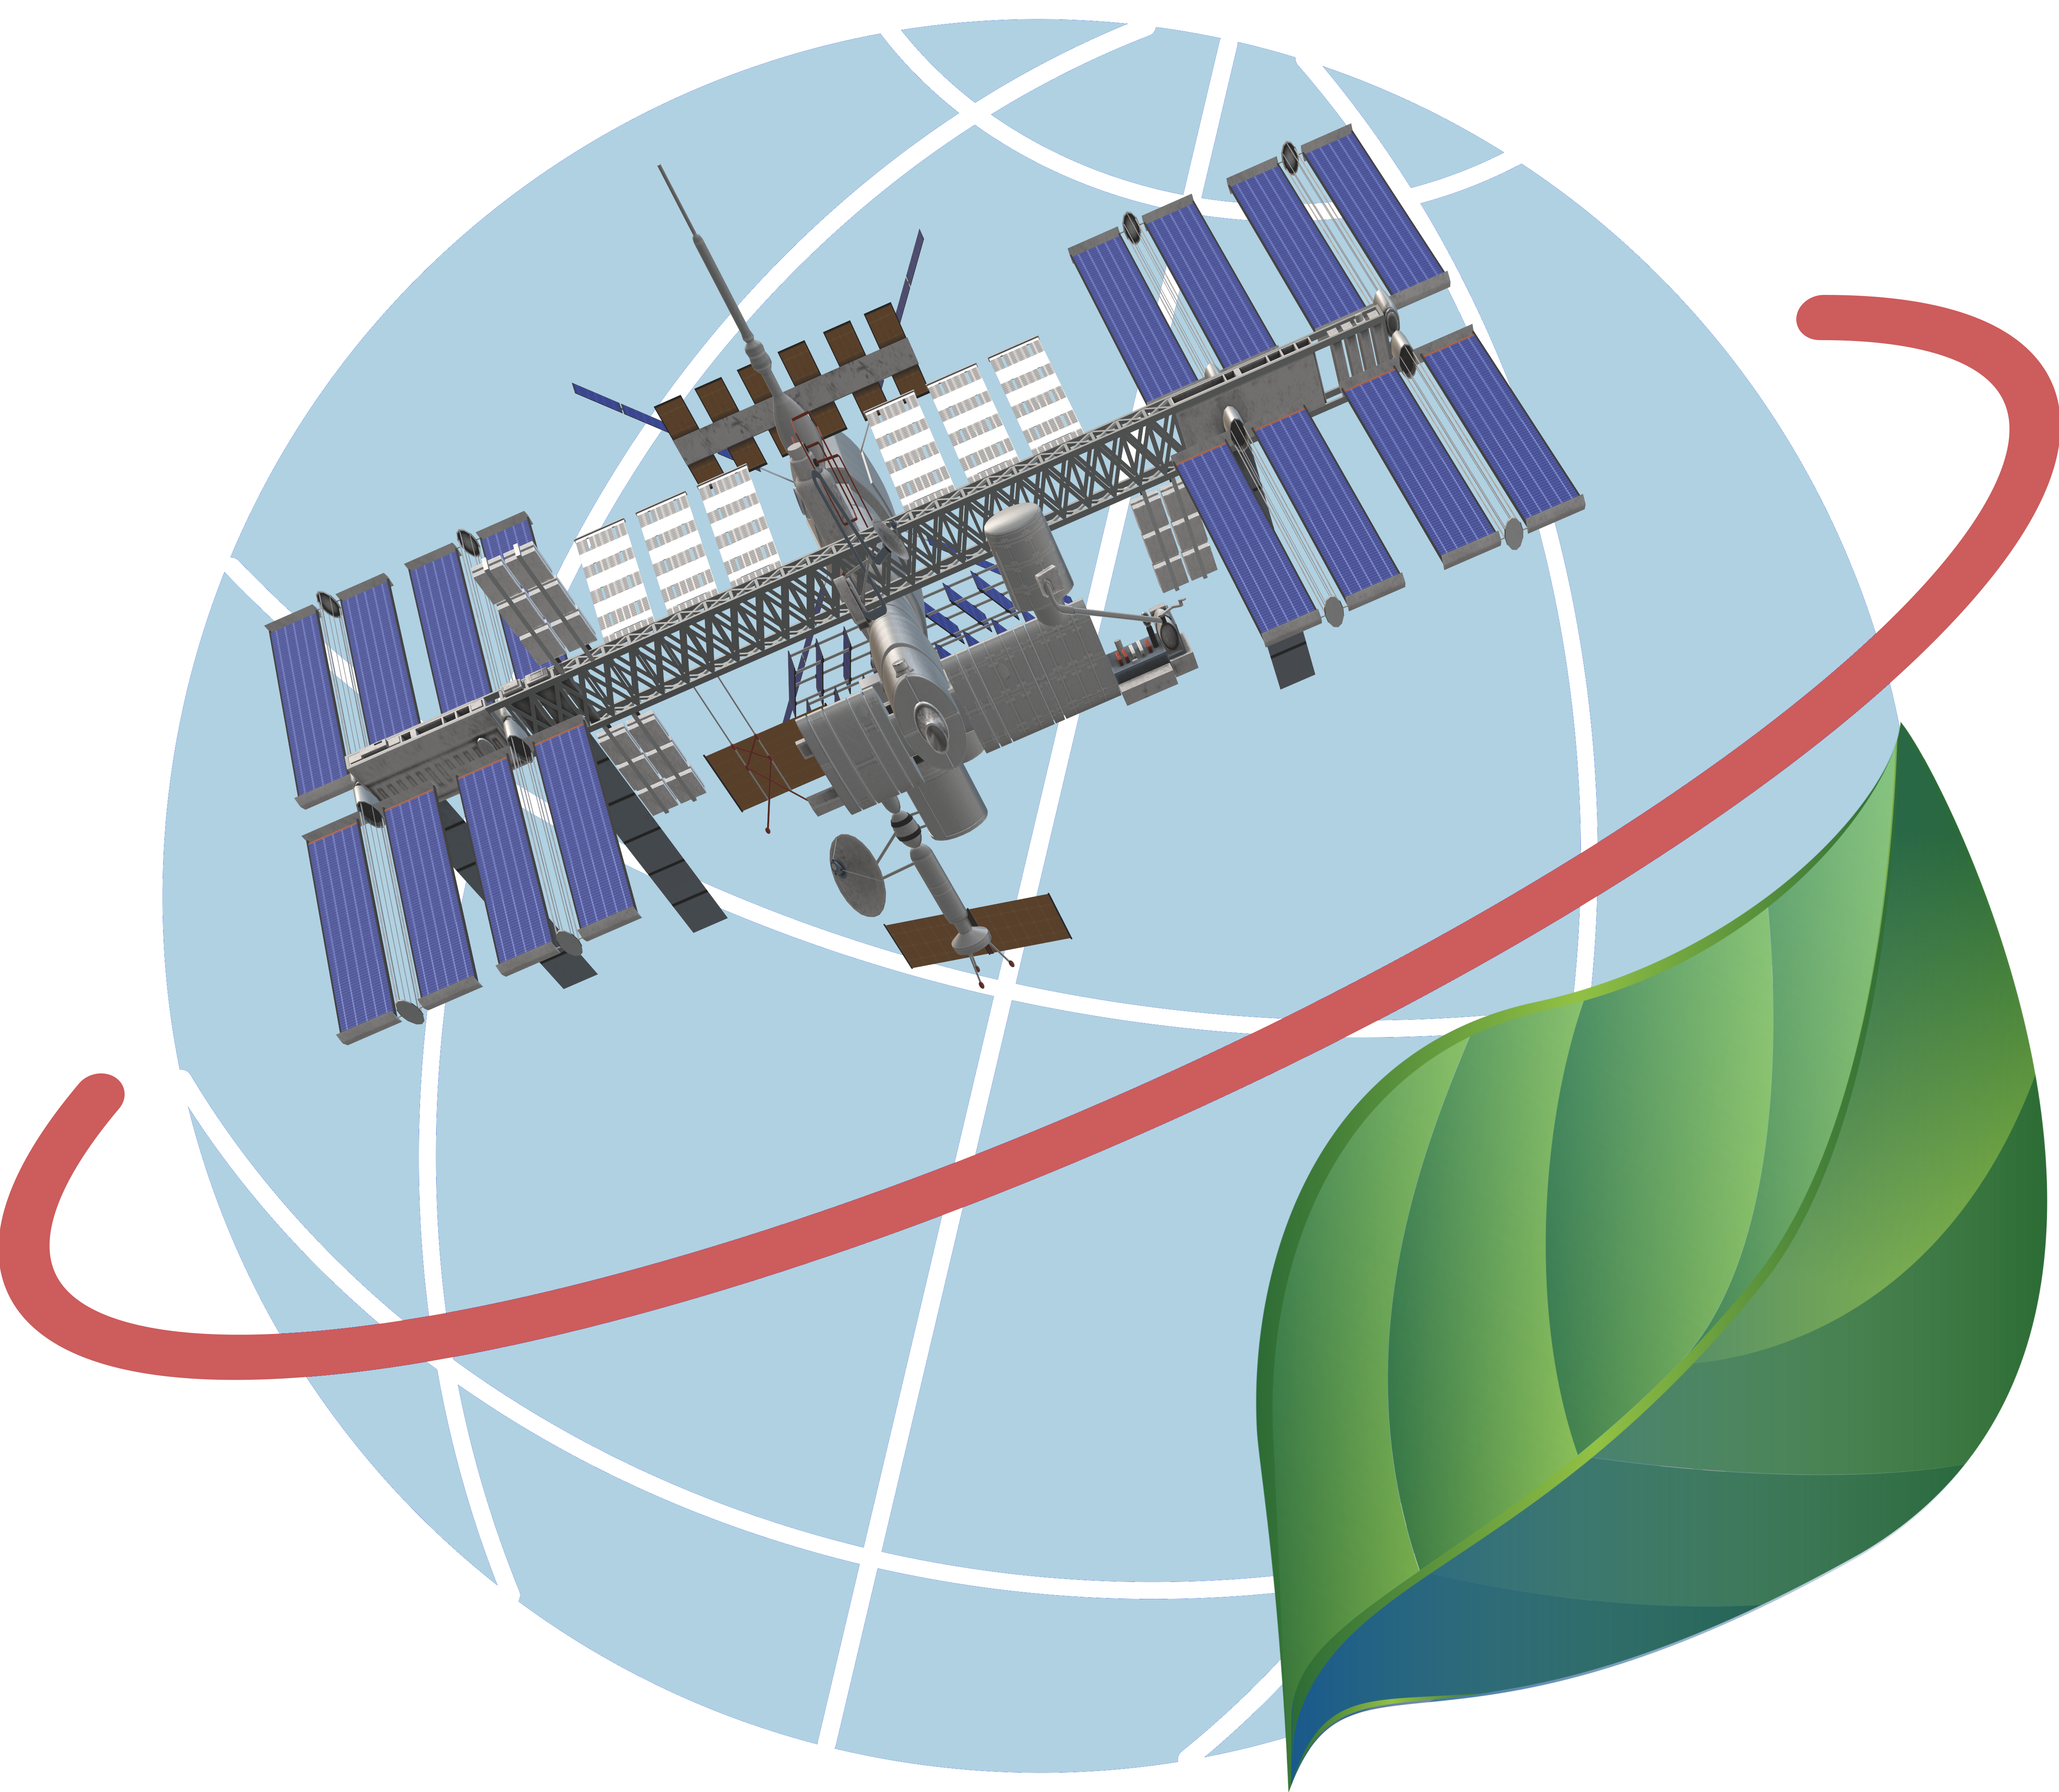
\includegraphics[scale=.125]{ICECREAM_Logo.png}};\end{tikzpicture}}
	%%%%%%%%%%%%%%%%%%%%%%%%%%%%%%%%%%
	
	\noindent\fbox{\begin{minipage}{.9665\textwidth}
			
			\vspace{1em}
			\begin{center}
				\textbf{\Large \underline{Motivation For Today's Tutorial : }}
			\end{center}
			
			\vspace{1 em}
			
			\centerline{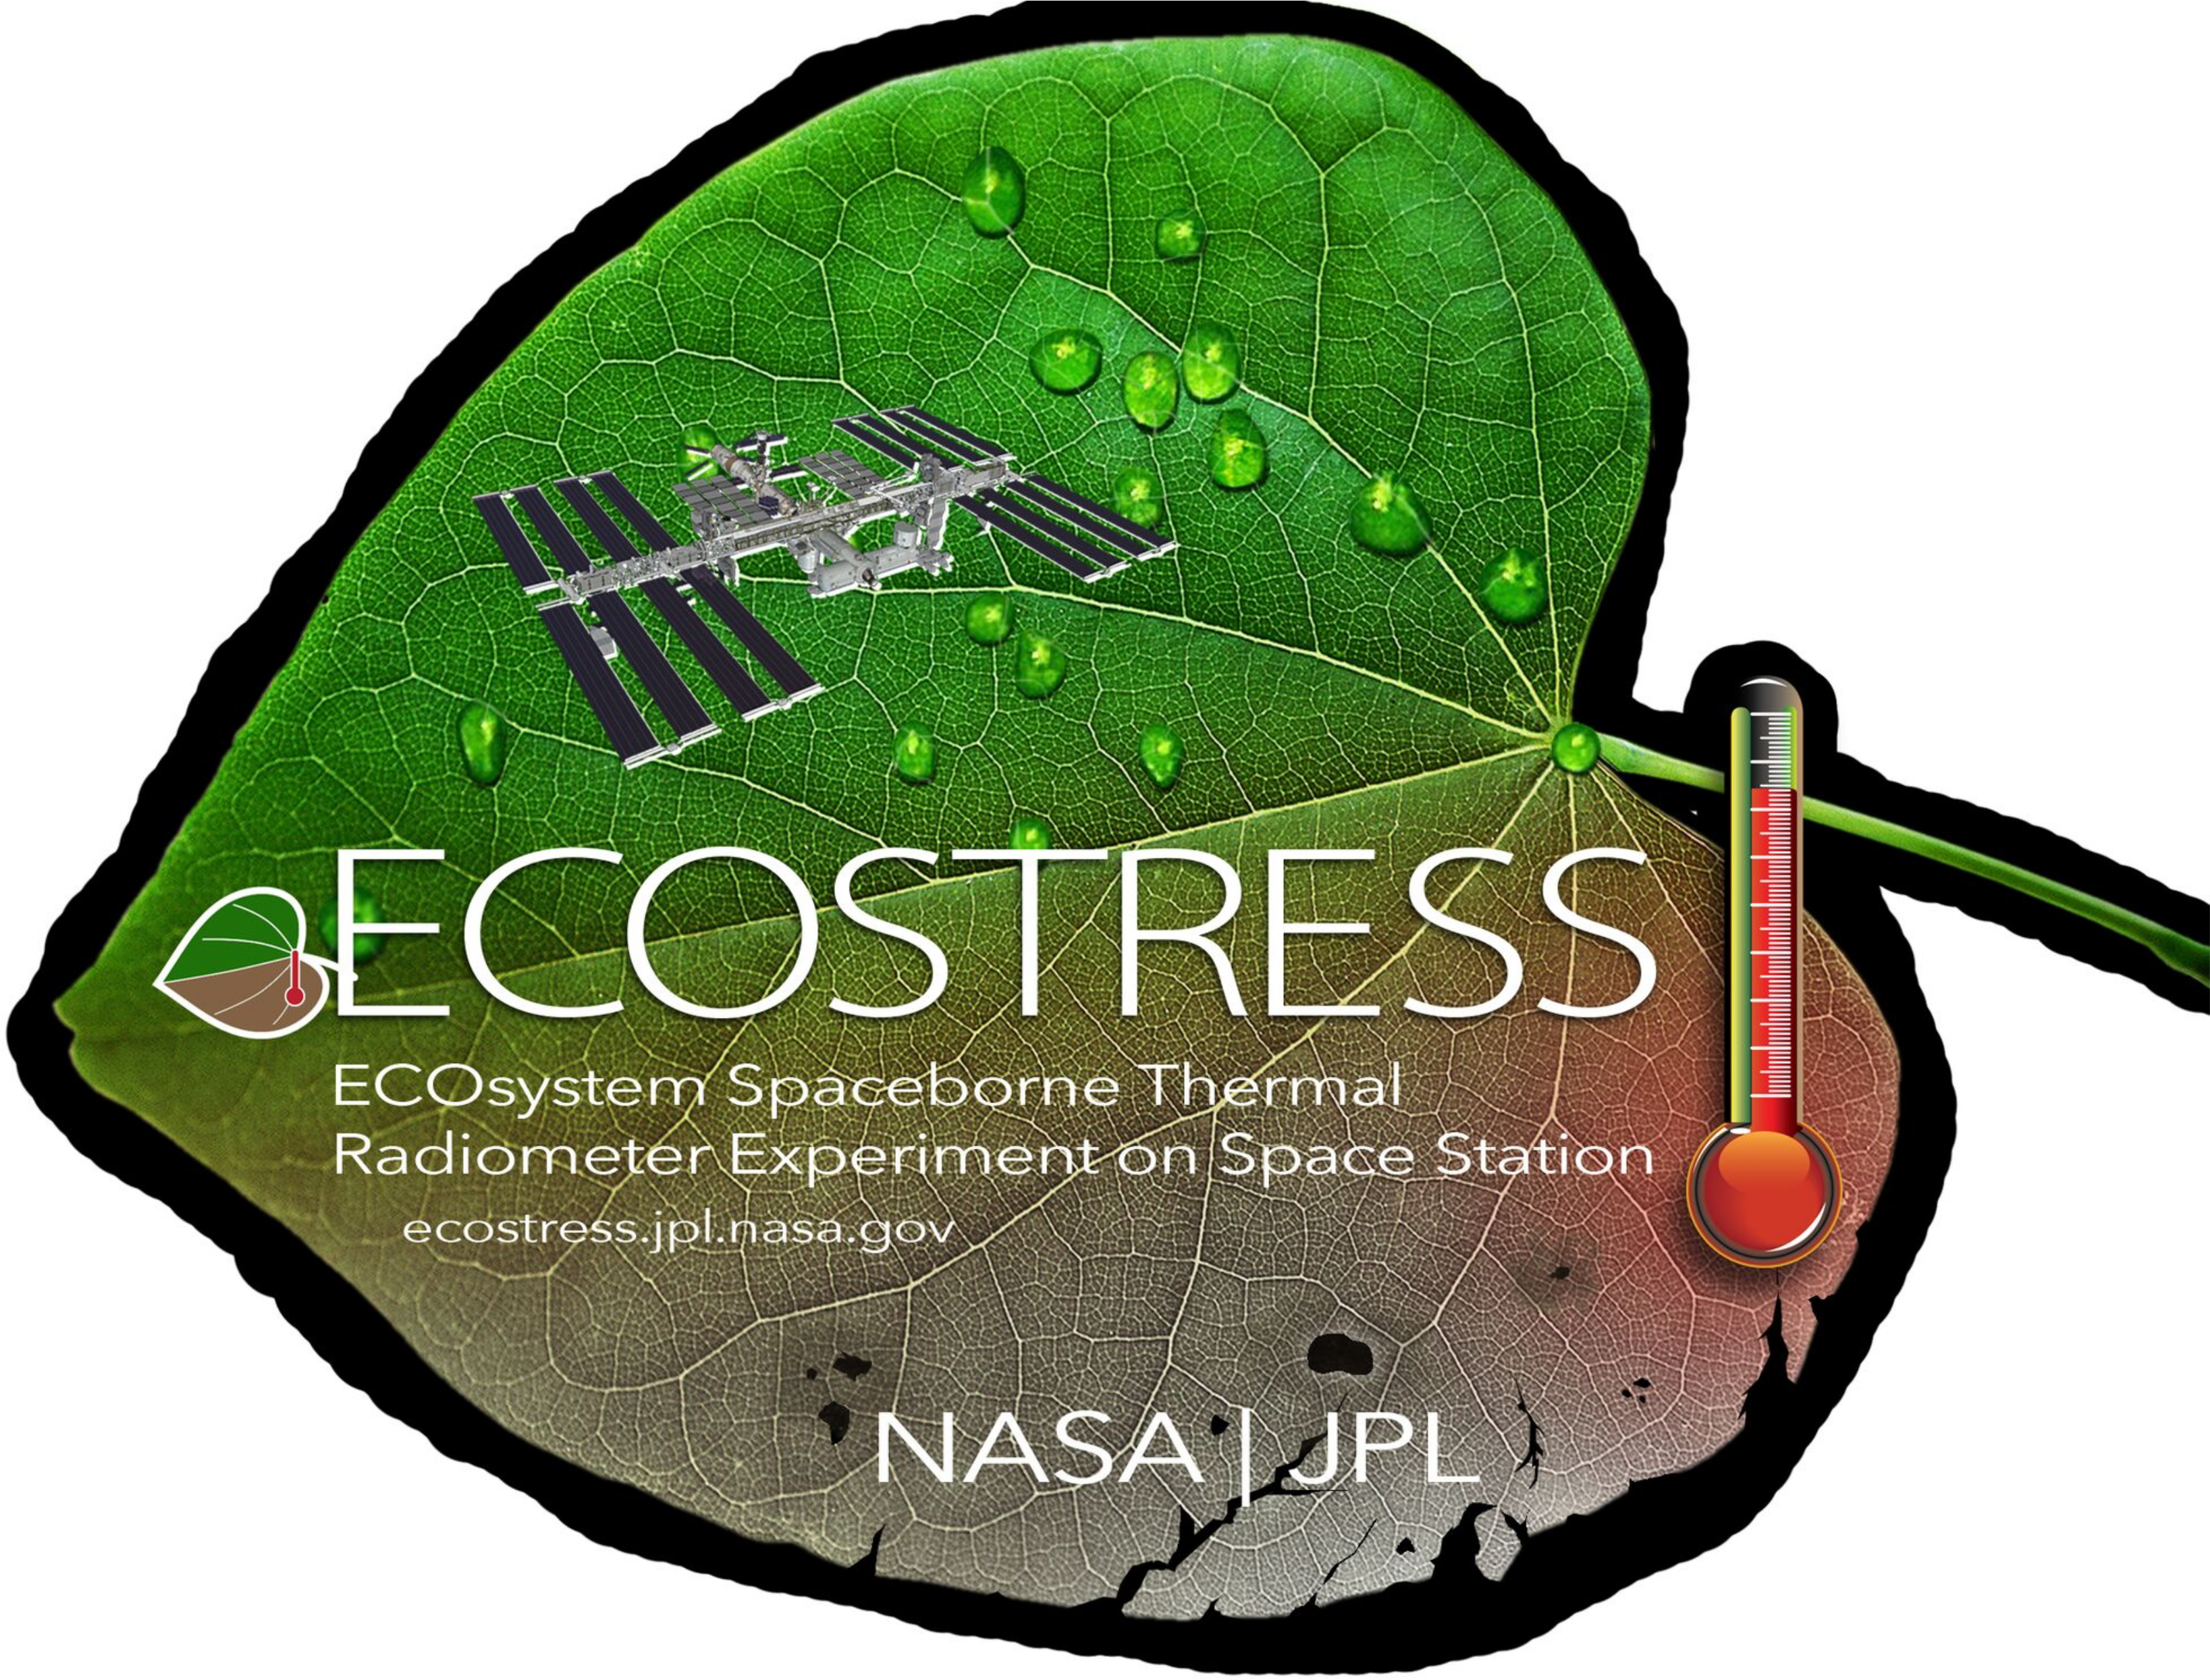
\includegraphics[width=.75\textwidth]{ECOSTRESS_Logo.png}}
			
			\vspace{1 em}
			
			
			The Motivation For The Tutorial Will Go Here
			
	\end{minipage}}
	
	\vspace{1 em}

\section{Section 1}

This is an example tutorial file with a custom theme for the ICECREAM Tutorials written by \href{https://www.jeremyforsythe.dev/}{Jeremy Forsythe}.

\section{Boxes Figures, and Images}

\subsection{Boxes}

\kulbox{{\bf Note:} This is an example of a Note Box.}

\begin{tcolorbox}[colback=yellow!5!white,colframe=IceCreamLeaf,title=\textbf{Box Title}]
	This is an example box.
\end{tcolorbox}

\subsection{Figures and Images}

You can reference figures like this (top)... See Figure: \ref{fig:ECOSTRESS_Logo}.

\begin{figure}[h]
    \centering
    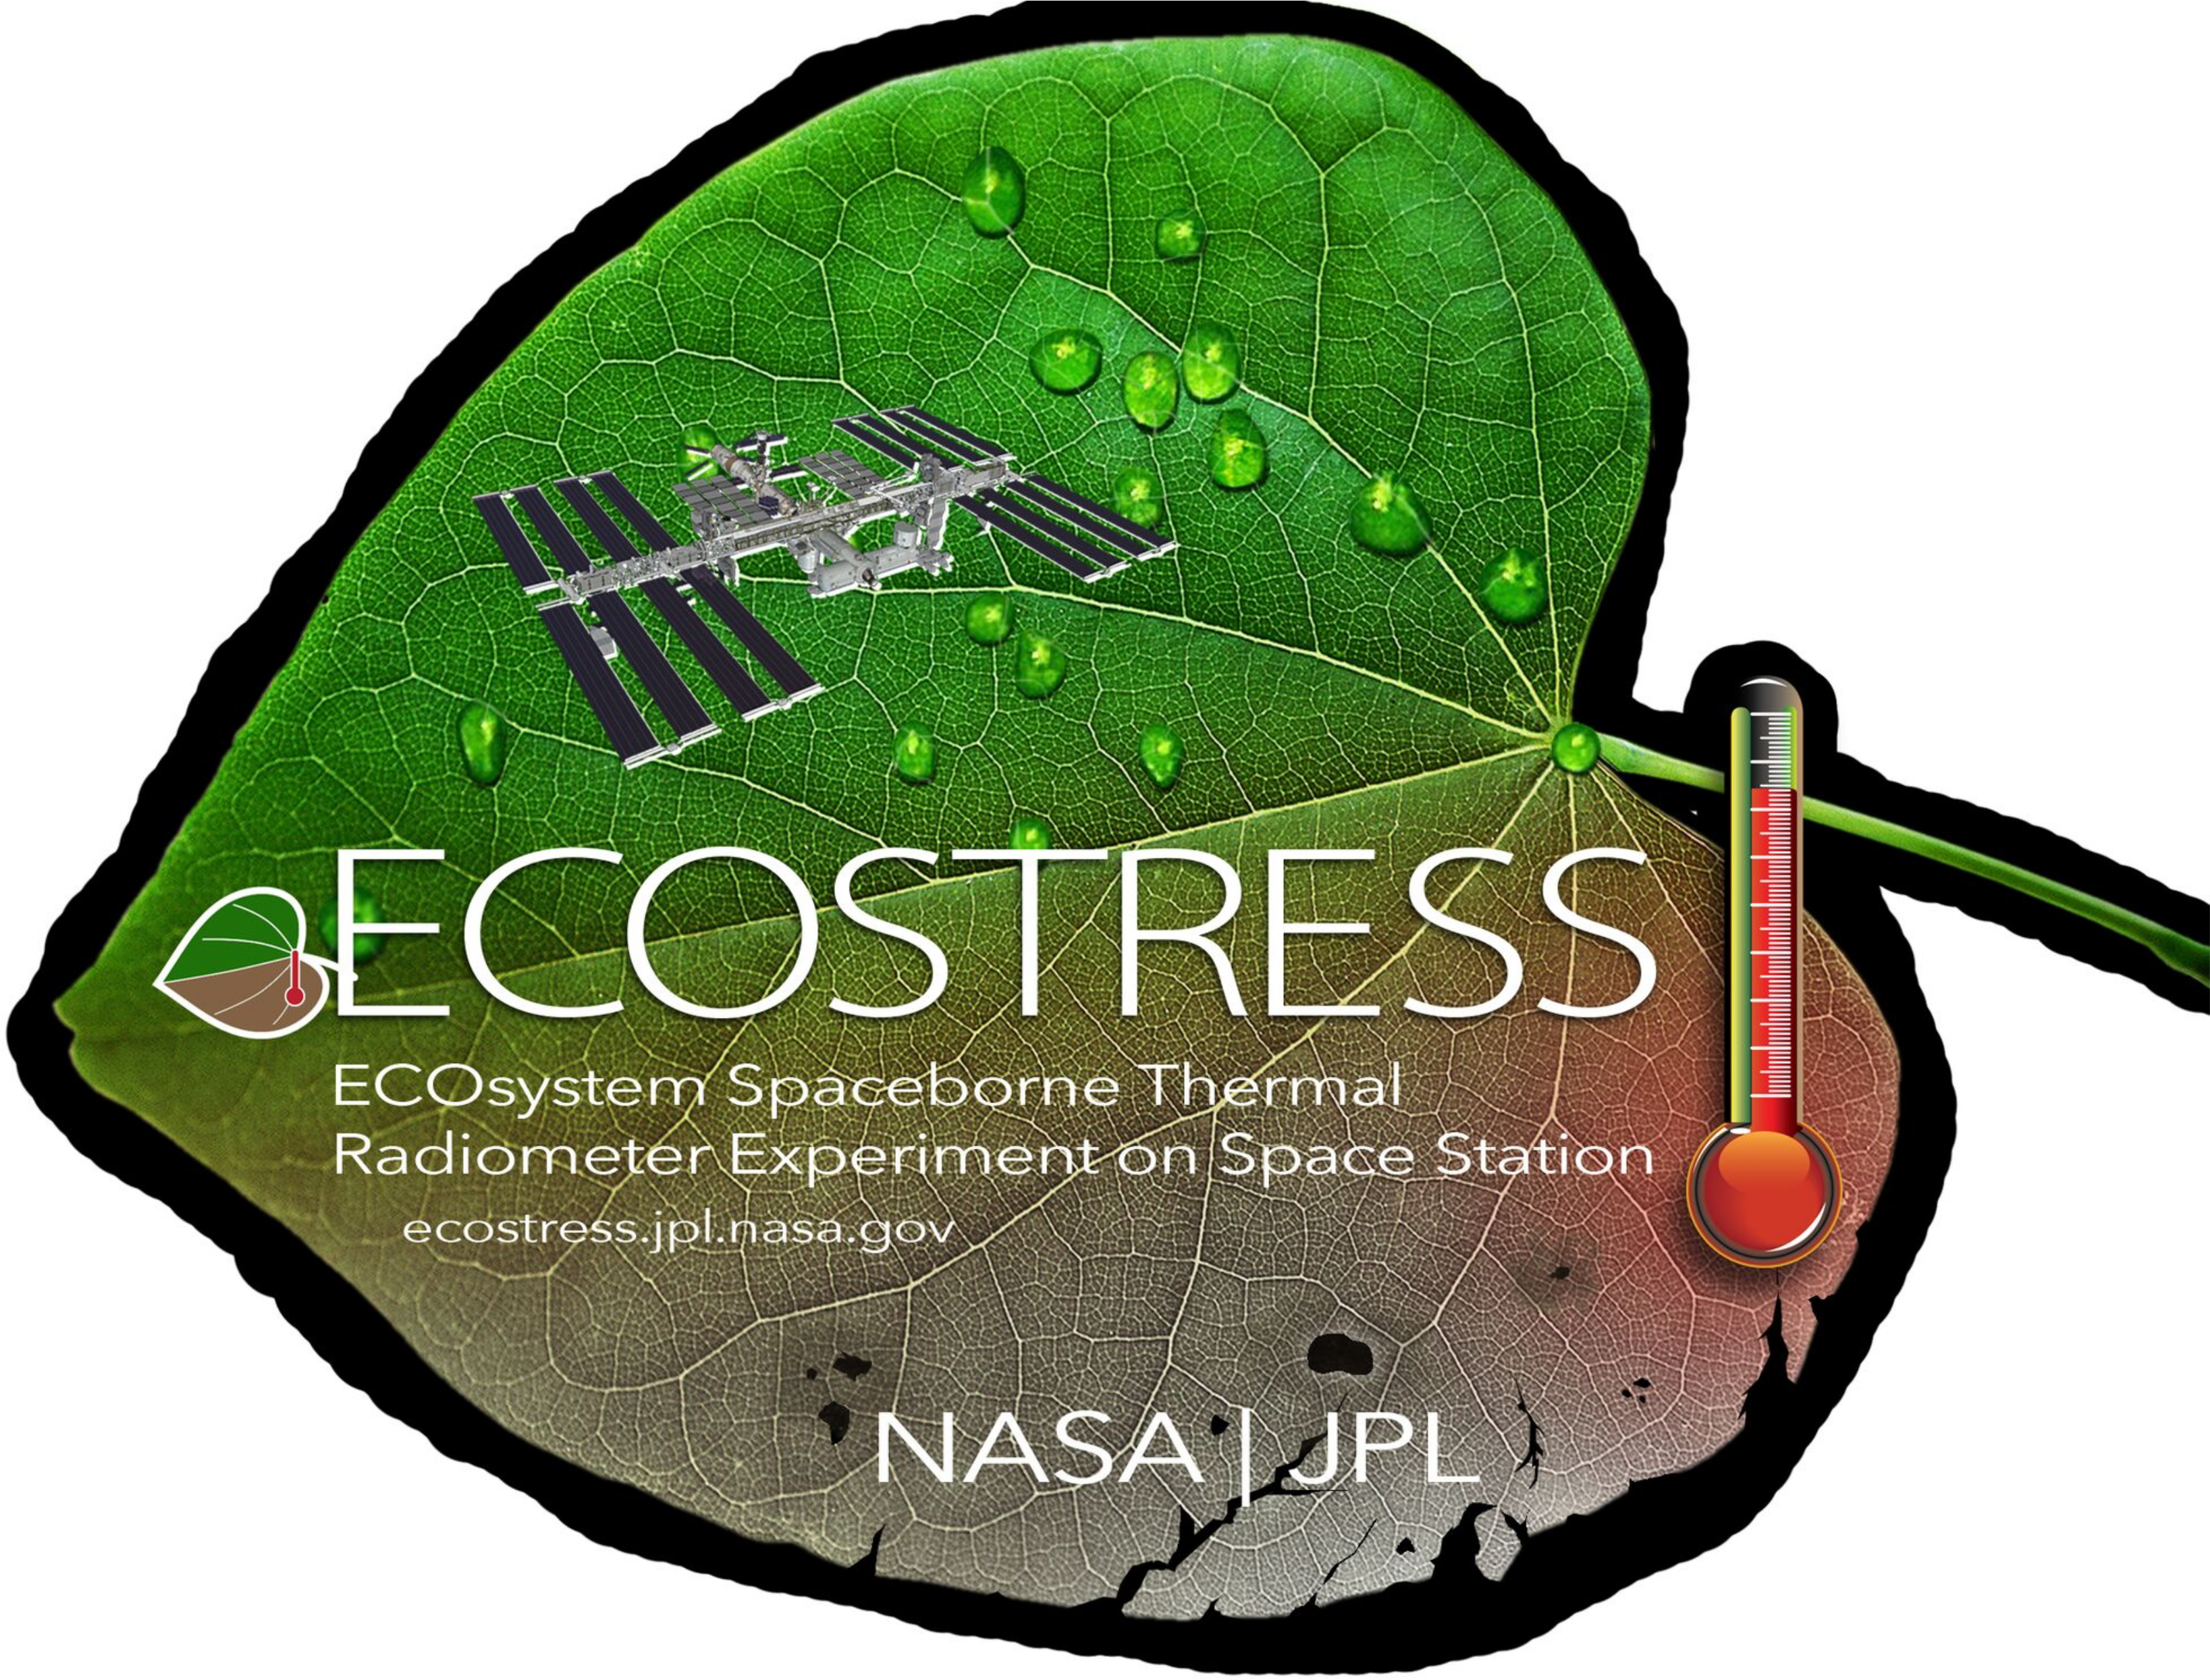
\includegraphics[width=.4\textwidth]{ECOSTRESS_Logo.png}
    \caption{The ECOSTESS Logo}
    \label{fig:ECOSTRESS_Logo}
\end{figure}

Images can also be included without making them a full on figure (bottom):

\centerline{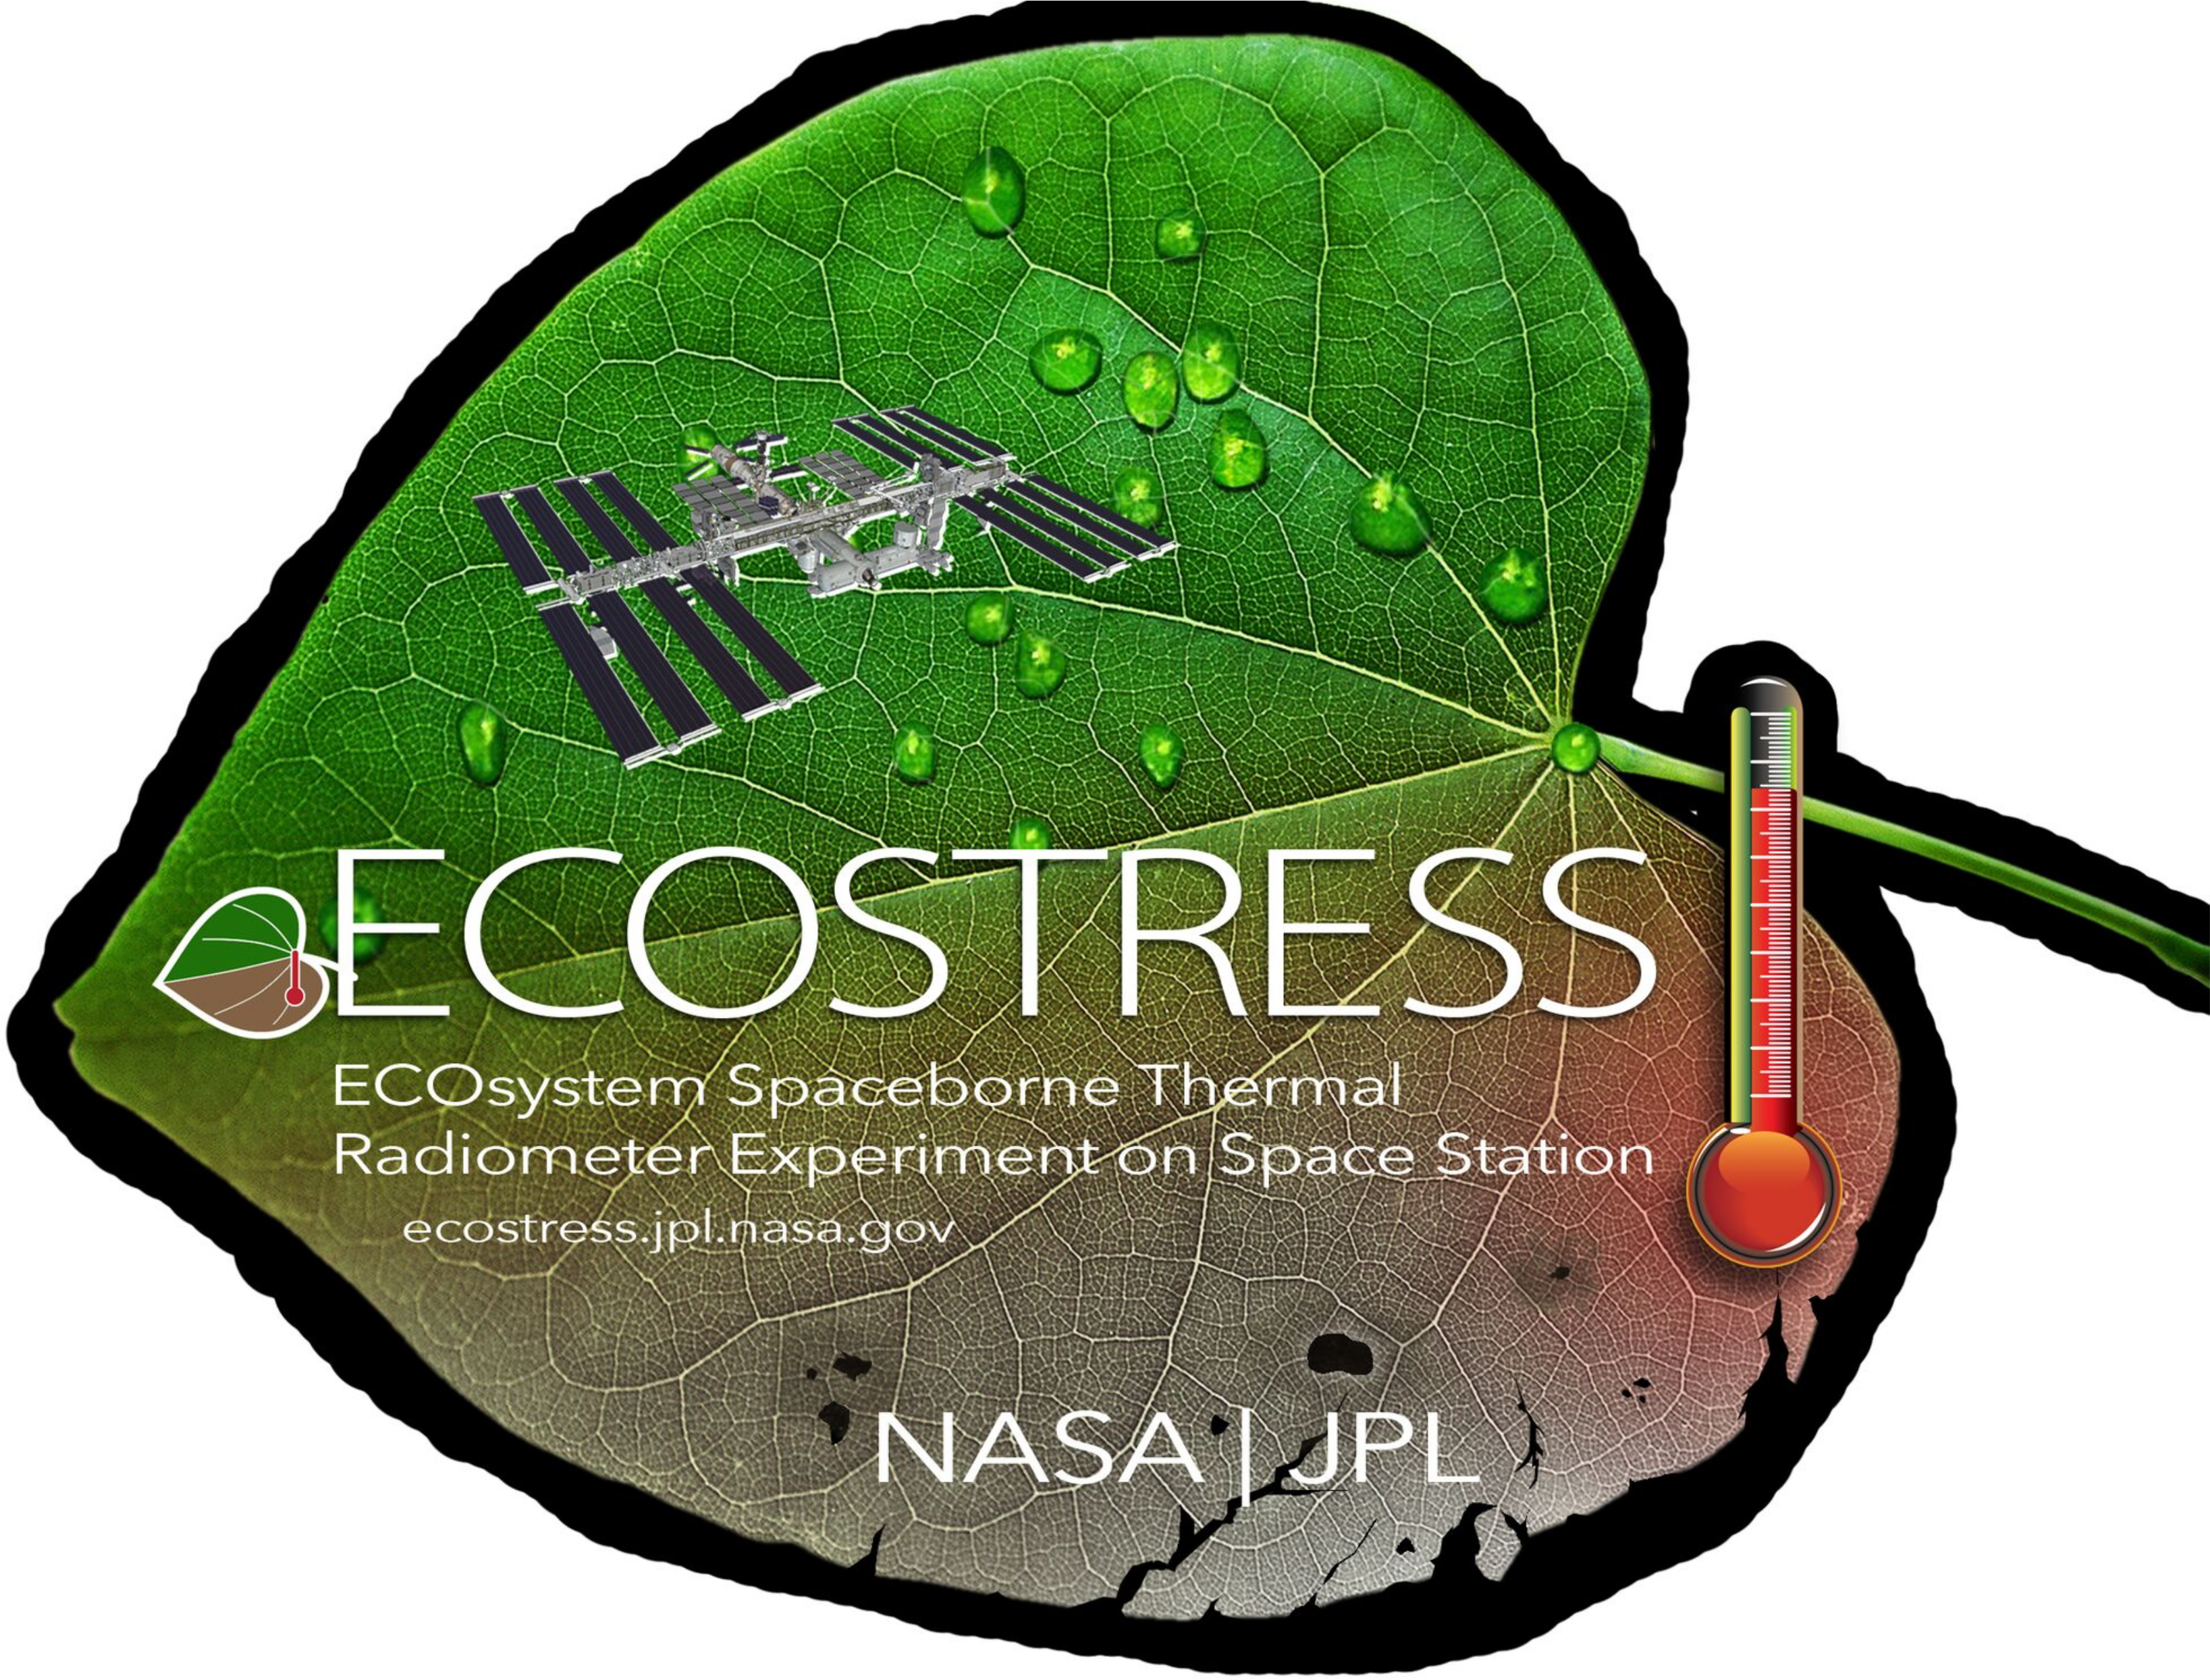
\includegraphics[width=.4\textwidth]{ECOSTRESS_Logo.png}}

\vspace{.25em}

\hrule

\vspace{1 em}

\begin{tcolorbox}[colback=yellow!5!white,colframe=IceCreamOrbit,title= \vspace{.2em} \Large Map of the Week Assignments]
	\addcontentsline{toc}{section}{Map of the Week Assignments}
	\large
	\begin{enumerate}
		\item Map of the Week Assignments Go Here
	\end{enumerate}	
	Submit these assignments via Canvas before Monday's class.
\end{tcolorbox}

\vspace{2 em}

\begin{tcolorbox}[title= \Large Datafiles]
	\addcontentsline{toc}{section}{Datafiles}
	\large
	In case any issues are encountered with the A$\rho\rho$EEARS database, data files used in the tutorial will be linked here:
	\begin{enumerate}
		\item \href{https://jeremydforsythe.github.io/icecream-tutorials/Tutorial2_AccessingRemoteSensingDataWithAppears/ECO2LSTE.001_SDS_LST_doy2023209214149_aid0001.tif}{ECO2LSTE.001\_SDS\_LST\_doy2023209214149\_aid0001.tif}
	\end{enumerate}
\end{tcolorbox}


%%%%%%%%%%%%%%%%%%%%%%%%%%%%%%%%%%%%%%%%%%%%%%%%%%%%%%%%%%%%%%%%%%%%%%%%%%%%%%%%%%% End of Document
\vfill

\hrule

\vspace{1em}

\textbf{Recommended Citation:} Forsythe, J.D., G.R. Goldsmith, and J.B. Fisher. 2023. Observing Earth from Above Tutorials. Chapman University. \url{https://jeremydforsythe.github.io/icecream-tutorials/}

\vspace{1em}

This work is supported by funding from NASA ECOSTRESS Mission Grant \#80NSSC23K0309 (I.C.E. C.R.E.A.M.: Integrating Communication of ECOSTRESS Into Community Research, Education, Applications, and Media).

\end{document}